\documentclass[10pt]{article}

% Language setting
% Replace `english' with e.g. `spanish' to change the document language
\usepackage[english]{babel}

% Set page size and margins
% Replace `letterpaper' with`a4paper' for UK/EU standard size
\usepackage[a4paper,top=2cm,bottom=2cm,left=3cm,right=3cm,marginparwidth=1.75cm]{geometry}

% Useful packages
\usepackage{amsmath}
\usepackage{tikz}
\usepackage{graphicx}
\usepackage{mwe}
\usepackage{fullpage}
\usepackage{hyperref}
\hypersetup{linkcolor=blue, urlcolor=blue, colorlinks}
\usepackage{caption}
\usepackage{subcaption}
\usepackage{float}
\usepackage{enumerate}

\title{Project: Sparse Matrix Formats \\ \large \textit{Accelerator-based Programming}}
\author{Oskar Tegby}
\date{October 2022}

\setlength{\parindent}{0pt}

\begin{document}
\maketitle

\begin{tikzpicture}[remember picture, overlay]
  \node [anchor=north west, inner sep=25pt]  at (current page.north west)
     {
\includegraphics[height=3.3cm]{uppsala-universitet-logo.png}};
\end{tikzpicture}

\section{Introduction}
This project studies the computational bandwidths of an iterative solver for a finite element problem using a data structure for sparse matrices called compressed row storage (CRS). To be specific, we study the computational throughput of a conjugate gradient method with a sparse matrix that comes from the finite element discretization of the Laplacian on a three-dimensional domain $(0,1)^3$ meshed with bricks. Notably, this problem is studied both on the processor using C++ and on the graphics card using CUDA. \\

All tests were run on the \href{https://www.uppmax.uu.se/resources/systems/the-snowy-cluster/}{Snowy} node of the UPPMAX cluster using a NVIDIA Tesla T4 graphics card, and an Intel Xeon E5-2660 processor, and repeated 50 times to reduce the noise in the measurements.

\section{Tasks}
This section addresses the grading criteria to pass the assignment one-by-one in order to clearly show that the required functionality and knowledge has been obtained.
\subsection{Criteria 1}
\subsubsection{Instruction}
\textit{Provide a correct program for the basic tasks involving the CRS matrix both on the CPU and the GPU.}
\subsubsection{Solution}
Please find the attached code. The correctness of these implementations is assured by observing that the error of the $\ell^2$ norm decreases by a factor four when doubling the problem size, $N$, when executing the code assignment
\begin{center}
    \texttt{/app.v -repeat 100 -number Number},
\end{center}
where \texttt{Number} refers to the datatype used, which is either \texttt{float} or \texttt{double}, and \texttt{v} refers to either the \texttt{host} or \texttt{cuda} code.
\subsection{Criteria 2}
\subsubsection{Instruction}
\textit{Provide computational measurements of acceptable performance on both platforms and display them in an understandable manner.}
\begin{figure}[!ht]
        \centering
    \begin{subfigure}[b]{0.49\textwidth}
        \centering
        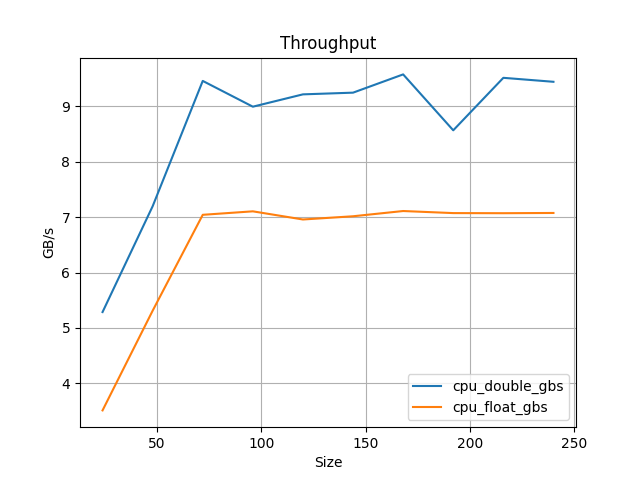
\includegraphics[width=\linewidth]{cpu_gbs.png}
        \caption{The CPU throughput in GB/s.}
        \label{fig:cpu_gbs}
    \end{subfigure}\hfill
    \begin{subfigure}[b]{0.49\textwidth}
        \centering
        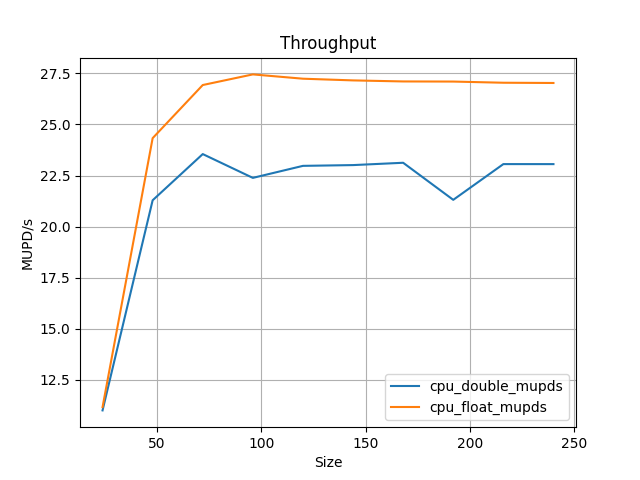
\includegraphics[width=\linewidth]{cpu_mupds.png}
        \caption{The CPU throughput in MUPD/s.}
        \label{fig:cpu_mupds}
    \end{subfigure}\hfill
    \caption{The throughput achieved on the CPU.}
    \label{fig:cpu}
\end{figure}
\begin{figure}[!ht]
        \centering
    \begin{subfigure}[b]{0.49\textwidth}
        \centering
        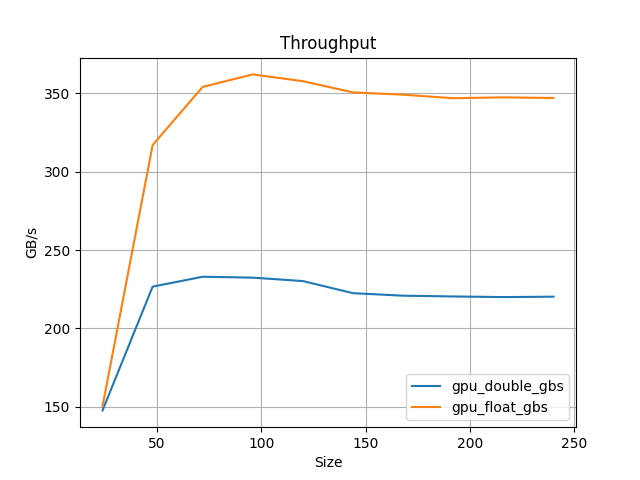
\includegraphics[width=\linewidth]{gpu_gbs.png}
        \caption{The GPU throughput in GB/s.}
        \label{fig:gpu_gbs}
    \end{subfigure}\hfill
    \begin{subfigure}[b]{0.49\textwidth}
        \centering
        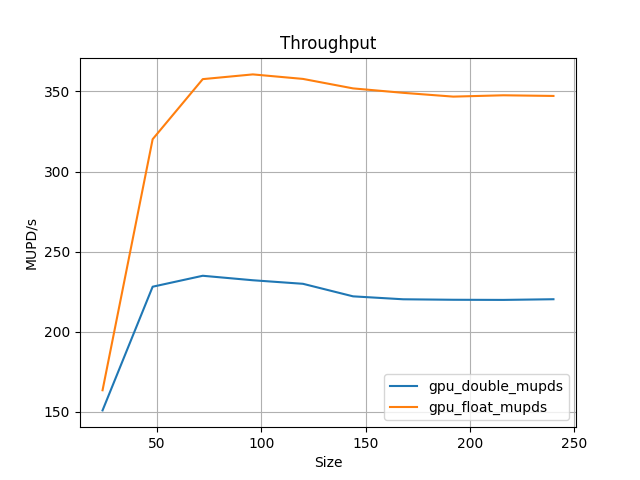
\includegraphics[width=\linewidth]{gpu_mupds.png}
        \caption{The GPU throughput in MUPD/s.}
        \label{fig:gpu_mupds}
    \end{subfigure}\hfill
    \caption{The throughput achieved on the GPU.}
    \label{fig:gpu}
\end{figure}
\subsection{Criteria 3}
\subsubsection{Instruction}
\textit{Provide explanations for the expected performance of the sparse matrix-vector product and conjugate gradient solver with basic CRS matrix storage as well as the improved ELLPACK/SELL-C-Sigma approach by Kreutzer et al.}
\subsubsection{Solution}
The performance with basic CRS storage is poor since the potential performance gained by vectorization and parallelization of the matrix-vector multiplication is ruined by the irregular data storage. That is solved by the ELLPACK storage, which fills all of the rows with zeros so that the rows are the same length. \\

However, that introduces the issue of storing a lot of unnecessary zeros, which is what CELL-C-$\sigma$ solves by locally sorting $\sigma$ rows of the data. That is, the data is sorted in groups of $\sigma$ elements. The C in SELL-C-$\sigma$ indicates how large the groups which are given extra zeros are. This decreases the number of zeros substantially, which improves performance without losing the ability to easily vectorize and parallelize the implementation on the GPU. \\

The expected performance increase should be about a factor two given the greatly decreased number of zeros stored in ELLPACK/SELL-C-$\sigma$.
\subsection{Criteria 4}
This section needs to be written.
\subsubsection{Instruction}
\textit{Discuss the topics of data both in the report and during oral discussion of the project.}
\subsubsection{Solution}
Please see Criteria 3.
\end{document}
